%  LaTeX support: latex@mdpi.com 
%  For support, please attach all files needed for compiling as well as the log file, and specify your operating system, LaTeX version, and LaTeX editor.

%=================================================================
\documentclass[journal,article,submit,pdftex,moreauthors]{Definitions/mdpi}

%=================================================================
% MDPI internal commands - do not modify
\firstpage{1} 
\makeatletter 
\setcounter{page}{\@firstpage} 
\makeatother
\pubvolume{1}
\issuenum{1}
\articlenumber{0}
\pubyear{2026}
\copyrightyear{2026}
%\externaleditor{Firstname Lastname} % More than 1 editor, please add `` and '' before the last editor name
\datereceived{ } 
\daterevised{ } % Comment out if no revised date
\dateaccepted{ } 
\datepublished{ } 
%\datecorrected{} % For corrected papers: "Corrected: XXX" date in the original paper.
%\dateretracted{} % For retracted papers: "Retracted: XXX" date in the original paper.
%\doinum{} % Used for some special journals, like molbank
%\pdfoutput=1 % Uncommented for upload to arXiv.org
%\CorrStatement{yes}  % For updates
%\longauthorlist{yes} % For many authors that exceed the left citation part
%\IsAssociation{yes} % For association journals

%=================================================================
% Add packages and commands here. The following packages are loaded in our class file: fontenc, inputenc, calc, indentfirst, fancyhdr, graphicx, epstopdf, lastpage, ifthen, float, amsmath, amssymb, lineno, setspace, enumitem, mathpazo, booktabs, titlesec, etoolbox, tabto, xcolor, colortbl, soul, multirow, microtype, tikz, totcount, changepage, attrib, upgreek, array, tabularx, pbox, ragged2e, tocloft, marginnote, marginfix, enotez, amsthm, natbib, hyperref, cleveref, scrextend, url, geometry, newfloat, caption, draftwatermark, seqsplit
% cleveref: load \crefname definitions after \begin{document}

%=================================================================
% Please use the following mathematics environments: Theorem, Lemma, Corollary, Proposition, Characterization, Property, Problem, Example, ExamplesandDefinitions, Hypothesis, Remark, Definition, Notation, Assumption
%% For proofs, please use the proof environment (the amsthm package is loaded by the MDPI class).

%=================================================================
% Full title of the paper (Capitalized)
\Title{Selective Falsification for Budget-Aware Self-Consistency in Chain-of-Thought Math Reasoning}

% Author Orchid ID: enter ID or remove command
\newcommand{\orcidauthorA}{0000-0000-0000-000X} % Add \orcidA{} behind the author's name
%\newcommand{\orcidauthorB}{0000-0000-0000-000X} % Add \orcidB{} behind the author's name

% Authors, for the paper (add full first names)
\Author{Firstname Lastname $^{1}$\orcidA{}, Firstname Lastname $^{2}$ and Firstname Lastname $^{2,}$*}

%\longauthorlist{yes}

% MDPI internal command: Authors, for metadata in PDF
\AuthorNames{Firstname Lastname, Firstname Lastname and Firstname Lastname}

% Affiliations / Addresses (Add [1] after \address if there is only one affiliation.)
\address{%
$^{1}$ \quad Affiliation 1; e-mail@e-mail.com\\
$^{2}$ \quad Affiliation 2; e-mail@e-mail.com}

% Contact information of the corresponding author
\corres{Correspondence: e-mail@e-mail.com; Tel.: (optional; include country code; if there are multiple corresponding authors, add author initials) +xx-xxxx-xxx-xxxx (F.L.)}

% Current address and/or shared authorship
%\firstnote{Current address: Affiliation.}
% Current address should not be the same as any items in the Affiliation section.

%\secondnote{These authors contributed equally to this work.}
% The commands \thirdnote{} till \eighthnote{} are available for further notes.

%\simplesumm{} % Simple summary

%\conference{} % An extended version of a conference paper

% Abstract (Do not insert blank lines, i.e. \\)
\abstract{Self-consistency (SC) improves chain-of-thought (CoT) reasoning by sampling multiple solutions and returning the most frequent final answer, but it implicitly treats sampled chains as exchangeable and uses popularity as a proxy for correctness. This can be brittle when a smaller or cost-constrained model repeatedly samples the same misconception, making the majority answer wrong. Confidence-weighted voting appears to address this but typically requires verifying every sampled chain and depends on self-reported confidence that can be poorly calibrated. We propose Selective Falsification-Weighted Self-Consistency (SFw-SC-CoT), a prompt-only aggregation rule that clusters sampled CoT outputs by unique final answer and verifies each answer hypothesis once with a deterministic ``try to disprove it'' checker. The checker performs three explicit sanity checks (estimation, alternative recomputation, and constraint checking) and outputs a confidence score and a checks-passed count. We combine down-weighted frequency with these falsification signals in a budget-aware scoring function. On GSM8K test problems ($N = 200$) with gpt-4o-mini and $K = 8$ sampled chains, SFw-SC-CoT increases accuracy from $0.93$ to $0.94$, while highlighting the need for improved compute logging to substantiate budget efficiency claims.}

% Keywords
\keyword{keyword 1; keyword 2; keyword 3 (List three to ten pertinent keywords specific to the article; yet reasonably common within the subject discipline.)}

% The fields PACS, MSC, and JEL may be left empty or commented out if not applicable
%\PACS{J0101}
%\MSC{}
%\JEL{}

%%%%%%%%%%%%%%%%%%%%%%%%%%%%%%%%%%%%%%%%%%
% Only for the journal Diversity
%\LSID{\url{http://}}

%%%%%%%%%%%%%%%%%%%%%%%%%%%%%%%%%%%%%%%%%%
% Only for the journal Applied Sciences
%\featuredapplication{Authors are encouraged to provide a concise description of the specific application or a potential application of the work. This section is not mandatory.}
%%%%%%%%%%%%%%%%%%%%%%%%%%%%%%%%%%%%%%%%%%

%%%%%%%%%%%%%%%%%%%%%%%%%%%%%%%%%%%%%%%%%%
% Only for the journal Data
%\dataset{DOI number or link to the deposited data set if the data set is published separately. If the data set shall be published as a supplement to this paper, this field will be filled by the journal editors. In this case, please submit the data set as a supplement.}
%\datasetlicense{License under which the data set is made available (CC0, CC-BY, CC-BY-SA, CC-BY-NC, etc.)}

%%%%%%%%%%%%%%%%%%%%%%%%%%%%%%%%%%%%%%%%%%
% Only for the journal BioTech, Fishes, Neuroimaging and Toxins
%\keycontribution{The breakthroughs or highlights of the manuscript. Authors can write one or two sentences to describe the most important part of the paper.}

%%%%%%%%%%%%%%%%%%%%%%%%%%%%%%%%%%%%%%%%%%
% Only for the journal Encyclopedia
%\encyclopediadef{For entry manuscripts only: please provide a brief overview of the entry title instead of an abstract.}

%%%%%%%%%%%%%%%%%%%%%%%%%%%%%%%%%%%%%%%%%%
% Different journals have different requirements. Please check the specific journal guidelines in the "Instructions for Authors" on the journal's official website.
%\addhighlights{yes}
%\renewcommand{\addhighlights}{%
%
%\noindent The goal is to increase the discoverability and readability of the article via search engines and other scholars. Highlights should not be a copy of the abstract, but a simple text allowing the reader to quickly and simplified find out what the article is about and what can be cited from it. Each of these parts should be devoted up to 2~bullet points.\vspace{3pt}\\
%\textbf{What are the main findings?}
% \begin{itemize}[labelsep=2.5mm,topsep=-3pt]
% \item First bullet.
% \item Second bullet.
% \end{itemize}\vspace{3pt}
%\textbf{What are the implications of the main findings?}
% \begin{itemize}[labelsep=2.5mm,topsep=-3pt]
% \item First bullet.
% \item Second bullet.
% \end{itemize}
%}

%%%%%%%%%%%%%%%%%%%%%%%%%%%%%%%%%%%%%%%%%%
\begin{document}

%%%%%%%%%%%%%%%%%%%%%%%%%%%%%%%%%%%%%%%%%%
\section{Introduction}

Chain-of-thought (CoT) prompting has become a standard inference-time technique for eliciting multi-step reasoning from large language models (LLMs) without fine-tuning. By prompting a model to ``solve step by step'' and produce intermediate natural-language reasoning, CoT can substantially improve performance on tasks that require multiple arithmetic or logical steps compared with directly prompting for the final answer, particularly at larger model scales \cite{wei-2022-chain}. At the same time, CoT does not guarantee correctness or faithfulness: a model can generate fluent reasoning that contains subtle arithmetic slips or incorrect assumptions, and stochastic decoding can produce different rationales and different answers for the same question \cite{wei-2022-chain}. This variability is especially consequential in settings where one seeks improved reliability without changing model weights, for example when only prompting is available.

Self-consistency (SC) is a widely used aggregation approach that attempts to stabilize CoT outcomes at inference time. Instead of trusting a single sampled chain, SC generates $K$ independent CoT samples and selects the most frequent extracted final answer via majority vote \cite{das-2022-self}. When errors are diverse and relatively uncorrelated, majority voting can outperform any single sample by amplifying the most probable correct solution path.

However, SC makes a strong implicit assumption: it treats sampled chains as exchangeable evidence and equates the frequency of an answer with its likelihood of being correct. This assumption becomes brittle when samples are correlated through shared misconceptions. In that regime, increasing $K$ can simply increase the frequency of the same wrong answer rather than revealing an alternative correct hypothesis. A seemingly natural extension is to weight each sample's vote by a confidence score obtained from a verifier prompt. In practice, such per-sample verification can (i) depend on self-reported confidence that may be miscalibrated, and (ii) increase compute because it adds an additional verifier call for each of the $K$ chains.

This paper targets a prompt-only gap: an aggregation rule that (a) is less sensitive to shared misconceptions than pure frequency voting by explicitly attempting falsification, and (b) can be more sample-efficient by verifying only a small number of answer hypotheses rather than verifying every sampled chain. We propose Selective Falsification-Weighted Self-Consistency (SFw-SC-CoT), a simple, inference-only algorithm that reframes SC as hypothesis testing. The method first samples $K$ CoT solutions, clusters them by unique extracted final answer, and then runs a deterministic verifier once per unique answer hypothesis. The verifier is asked to try to disprove the hypothesis using three explicit sanity checks: a magnitude estimate, an alternative recomputation, and a constraint check based on the problem statement. It outputs two structured signals: a confidence $c(a) \in [0,1]$ and a discrete checks-passed count $p(a) \in \{0,1,2,3\}$. We then select the answer with the highest score under a budget-aware aggregation rule that down-weights frequency so that popularity alone cannot dominate.

We evaluate SFw-SC-CoT using the provided codebase on GSM8K test problems. In the executed experiment, both baseline SC and SFw-SC-CoT use the same generation budget ($K = 8$ CoT samples, temperature $0.7$, max\_tokens $512$) and the same model (gpt-4o-mini). The baseline uses majority voting over extracted answers; the proposed method performs answer-level falsification verification and weighted aggregation. On $N = 200$ GSM8K test problems, the proposed method achieves $0.94$ accuracy ($188/200$) compared with $0.93$ ($186/200$) for SC.

\subsection{Contributions}
\begin{itemize}
\item \textbf{Selective falsification aggregation.} We propose SFw-SC-CoT, a prompt-only aggregation method that verifies answer hypotheses rather than individual chains, using structured falsification prompts.
\item \textbf{Budget-aware scoring rule.} We introduce a scoring rule that combines down-weighted frequency with two verifier-derived signals (confidence and checks passed).
\item \textbf{End-to-end evaluation.} We provide an end-to-end evaluation on GSM8K ($N = 200$) with gpt-4o-mini at fixed $K = 8$, showing a small positive accuracy improvement and reporting the corresponding runtime difference.
\end{itemize}

The current results are intentionally narrow, reflecting what was actually executed and logged. Future work should extend the evaluation across additional $K$ values and datasets, and, crucially, log hypothesis counts and token usage so that accuracy can be assessed under explicit compute budgets rather than only under fixed sampling parameters.

%%%%%%%%%%%%%%%%%%%%%%%%%%%%%%%%%%%%%%%%%%
\section{Related Work}

CoT prompting is a foundational inference-time method for improving multi-step reasoning performance in LLMs without weight updates \cite{wei-2022-chain}. Its primary relevance to our setting is twofold. First, it provides the mechanism for producing explicit intermediate reasoning steps that often help models solve arithmetic word problems. Second, it exposes a reliability issue: models may produce plausible but incorrect reasoning traces, and stochastic generation can lead to multiple distinct solutions and answers for the same input \cite{wei-2022-chain}. These properties motivate aggregation methods that can exploit diversity across samples.

Self-consistency (SC) is a prominent aggregation strategy that samples multiple CoT chains and returns the most frequent final answer \cite{das-2022-self}. Relative to single-shot CoT, SC trades additional inference compute for improved robustness to decoding randomness. The key assumption is that the correct solution path is sampled more often than any particular incorrect path; under this assumption, majority vote increases the probability of returning the correct answer.

Our work is closest to SC but differs in both the evidential model and the compute allocation. SC effectively assumes exchangeability of sampled chains: each chain contributes one unit vote, and frequency is the sole criterion for selection. This makes SC vulnerable when samples share a systematic misconception, because correlated errors can become the majority. SFw-SC-CoT modifies the SC pipeline by treating distinct final answers as hypotheses and introducing an explicit falsification-oriented verification step at the hypothesis level. Instead of verifying each chain (which would scale verification compute linearly with $K$), we verify each unique answer hypothesis. This design aims to reduce the number of verifier calls from $K$ to $U$, where $U$ is the number of distinct extracted answers observed among the $K$ samples.

SFw-SC-CoT also differs from confidence-weighted voting schemes that rely only on self-reported confidence. While both our method and confidence weighting can be implemented via prompting, the falsification prompt used in SFw-SC-CoT constrains the verifier to perform three independent sanity checks and to report a discrete checks-passed signal alongside a continuous confidence score. The intent is to make verification less dependent on a single unconstrained confidence statement and to encourage error-search behavior similar to hypothesis testing.

In the present work, our empirical comparison is limited to SC majority vote, because only that baseline was executed and logged in the available experiments. Therefore, the primary contribution of the related-work comparison is conceptual: SFw-SC-CoT can be interpreted as an SC-style sampler with an additional hypothesis-level verification stage designed to mitigate correlated error modes that frequency alone cannot resolve.

%%%%%%%%%%%%%%%%%%%%%%%%%%%%%%%%%%%%%%%%%%
\section{Background}

This work focuses on multi-step math word problems where the desired output is a single numeric answer. The overall pipeline consists of chain-of-thought generation, extraction and normalization of numeric answers, aggregation across multiple samples, and (for the proposed method) verification signals derived from a falsification-style prompt.

\subsection{Problem setting and notation}
Let $q$ denote a natural-language problem. A stochastic CoT generator produces $K$ samples. Each sample $i$ yields a rationale $r_i$ (the generated reasoning text) and an extracted final numeric answer $a_i$. Samples are grouped by identical extracted answers. For any candidate answer string $a$, define $G(a)$ as the set of rationales that end in $a$, that is, $G(a) = \{ r_i : a_i = a \}$. Let $U$ be the number of unique answers with non-empty groups.

\subsection{Baseline self-consistency}
Standard SC aggregates by majority vote over extracted final answers, returning $\arg\max_a |G(a)|$ \cite{das-2022-self}. In effect, it estimates that an answer is correct if it is sampled most frequently among the $K$ chains.

\subsection{Answer extraction and normalization}
The implementation extracts a final numeric answer from a rationale using a prioritized list of regular expressions. These patterns are designed to handle common answer formats observed in practice, including GSM8K-style ``\#\#\#\# 42'', explicit ``Answer:'' phrases, markdown bold numbers, and boxed answers, with a final permissive fallback that selects the last number appearing in the text. Ground-truth labels are extracted from GSM8K solutions primarily using the ``\#\#\#\#'' delimiter. For evaluation, predicted and ground-truth answers are normalized by removing commas, stripping certain symbols such as ``\$'', removing spaces, and converting to a canonical numeric string so that integer and decimal representations (for example, ``5'' and ``5.0'') compare as equal.

\subsection{Answer-hypothesis verification signals}
SFw-SC-CoT introduces verification at the level of answer hypotheses. For each candidate answer $a$, a verifier prompt is constructed from the problem $q$, the proposed answer $a$, and up to $L$ representative rationales from $G(a)$. Representatives are selected by sorting rationales by length and choosing the shortest ones, reducing prompt length and limiting reliance on a single verbose chain. The verifier is instructed to attempt falsification via three sanity checks: (1) estimation or order-of-magnitude reasoning, (2) a brief alternative recomputation, and (3) a constraint check for consistency with the problem statement. The verifier output is parsed to obtain two scalars: confidence $c(a) \in [0,1]$ and checks\_passed $p(a) \in \{0,1,2,3\}$. These signals serve as inputs to the proposed aggregation rule.

%%%%%%%%%%%%%%%%%%%%%%%%%%%%%%%%%%%%%%%%%%
\section{Method}

SFw-SC-CoT modifies standard self-consistency by adding a falsification-oriented verification stage at the answer-hypothesis level. The method is inference-only and prompt-only: it uses no fine-tuning, no external tools, and no additional training data.

Given a problem $q$, the method proceeds as follows.

First, it samples $K$ chain-of-thought completions with stochastic decoding, producing rationales $r_1,\ldots,r_K$. In the provided implementation, the CoT prompt requests step-by-step reasoning and the sampling uses temperature $0.7$ with a fixed maximum generation length (max\_tokens). For each rationale $r_i$, we extract a final numeric answer $a_i$ with regex-based parsing.

Second, it forms answer hypotheses by grouping rationales that share the same extracted final answer. For each unique answer $a$, we obtain a group $G(a)$ of supporting rationales. Let $U$ be the number of unique extracted answers among the $K$ samples.

Third, it verifies each answer hypothesis once using a deterministic verifier prompt (temperature $0.0$). For each candidate answer $a$, the verifier is shown (i) the original problem $q$, (ii) the proposed answer $a$, and (iii) up to $L$ representative rationales from $G(a)$, selected as the shortest rationales in that group. The verifier is explicitly instructed to try to DISPROVE the proposed answer using exactly three independent sanity checks: magnitude or estimation, an alternative quick recomputation, and a constraint check (such as bounds, parity, or story consistency). The verifier response is parsed to obtain: (1) confidence $c(a)$, a real number in $[0,1]$; and (2) checks\_passed $p(a)$, an integer in $\{0,1,2,3\}$.

Fourth, it computes a score for each hypothesis and returns the highest-scoring answer. The aggregation rule is multiplicative and exponentiated:
\[
\mathrm{score}(a) = \left(\frac{|G(a)|}{K}\right)^{\alpha} \cdot \left(c(a)\right)^{\beta} \cdot \left(\frac{p(a)}{3}\right)^{\gamma}.
\]
In the executed proposed configuration, $\alpha = 0.5$, $\beta = 1.0$, and $\gamma = 1.0$. Compared with SC majority vote (which corresponds to $\alpha = 1$ and omits verification terms), this choice down-weights the impact of raw frequency so that a frequent hypothesis can be penalized if it fails falsification checks or receives low verifier confidence. The checks\_passed term is normalized by $3$ to map it into $[0,1]$. If parsing fails, the parser defaults checks\_passed to $0$ and confidence to $0.5$ and clips both to valid ranges.

The key design choice is verifying answer hypotheses rather than individual chains. Whereas per-chain verification would require $K$ verifier calls, SFw-SC-CoT requires $U$ verifier calls. The method therefore targets settings in which $K$ samples collapse to a small number of distinct answers, so that selective verification can focus compute on discriminating among hypotheses rather than scoring every chain.

\begin{algorithm}[H]
\caption{SFw-SC-CoT (Selective Falsification-Weighted Self-Consistency)}
\begin{algorithmic}[1]
\State \textbf{Input:} problem $q$, sampler, verifier, sample count $K$, reps limit $L$, exponents $\alpha,\beta,\gamma$
\State Sample CoT rationales $\{r_i\}_{i=1}^K$ with stochastic decoding
\State Extract answers $a_i \leftarrow \mathrm{Extract}(r_i)$ for $i \in \{1,\ldots,K\}$
\State Group rationales by answer: $G(a) \leftarrow \{r_i : a_i = a\}$ for each unique $a$
\For{each unique answer $a$}
  \State Select representatives $R(a) \leftarrow$ shortest $\min(L, |G(a)|)$ rationales from $G(a)$
  \State $(c(a), p(a)) \leftarrow \mathrm{Verify}(q, a, R(a))$ \Comment{deterministic, falsification checks}
  \State $s(a) \leftarrow \left(\frac{|G(a)|}{K}\right)^{\alpha} \cdot \left(c(a)\right)^{\beta} \cdot \left(\frac{p(a)}{3}\right)^{\gamma}$
\EndFor
\State \textbf{Return} $\arg\max_a s(a)$
\end{algorithmic}
\end{algorithm}

%%%%%%%%%%%%%%%%%%%%%%%%%%%%%%%%%%%%%%%%%%
\section{Experimental Setup}

We evaluate SFw-SC-CoT against a standard self-consistency baseline on GSM8K. This section describes only the experimental conditions that were actually executed and recorded in the provided run configurations and Weights and Biases (WandB) summaries.

\subsection{Task and dataset}
The task is to answer multi-step math word problems with a single numeric output. We use the GSM8K dataset, main subset, test split. The dataset is loaded via the HuggingFace datasets interface under the identifier \texttt{openai/gsm8k} with subset \texttt{main}. The run configuration sets max\_samples to $200$, and the logs indicate that exactly $N = 200$ test problems were processed.

\subsection{Model and access method}
Both baseline and proposed methods use the same model: gpt-4o-mini with base\_model gpt-4o-mini-2024-07-18 accessed through the OpenAI chat completions API. The codebase wraps the API in an \texttt{LLMModel} class that issues a separate generation call for each prompt.

\subsection{Generation and sampling protocol}
For each problem, both methods generate $K = 8$ chain-of-thought samples using temperature $0.7$ and max\_tokens $512$. Inference uses batch\_size $1$. Each completion is post-processed using the \texttt{extract\_final\_answer} function described in the Background section.

\subsection{Methods compared}
\textbf{Baseline SC majority vote.} Verification is disabled. After sampling and answer extraction, the baseline selects the answer with the largest group size $|G(a)|$. In the configuration, aggregation parameters are $\alpha = 1.0$, $\beta = 0.0$, and $\gamma = 0.0$, representing frequency-only aggregation.

\textbf{Proposed SFw-SC-CoT.} Verification is enabled. For each unique answer hypothesis $a$, the method runs a deterministic verifier (temperature $0.0$) using a falsification prompt. The verifier receives at most $L = 2$ representative rationales per hypothesis (max\_rationales\_per\_hypothesis $= 2$), chosen as the shortest rationales in that group. The parsed verifier outputs provide confidence and checks\_passed signals that are combined with frequency using $\alpha = 0.5$, $\beta = 1.0$, and $\gamma = 1.0$.

\subsection{Evaluation metric}
The primary metric is exact-match accuracy of the final numeric answer. Predictions and labels are normalized as described in Background, and a prediction is counted correct if the normalized strings match.

\subsection{Logging and artifacts}
Both runs log cumulative accuracy, num\_correct, and num\_total to WandB. The evaluation script fetches run summaries and produces four PDF figures: one per-run accuracy trace for each method and two comparison plots across methods.

%%%%%%%%%%%%%%%%%%%%%%%%%%%%%%%%%%%%%%%%%%
\section{Results}

This section reports the logged results from the executed GSM8K runs. No additional datasets, $K$ values, or baselines beyond those described in Experimental Setup were run, and we do not report any unlogged measurements.

\subsection{Overall accuracy on GSM8K}
On $N = 200$ test problems with $K = 8$, the SC baseline achieves accuracy $0.93$, corresponding to $186$ correct out of $200$. SFw-SC-CoT achieves accuracy $0.94$, corresponding to $188$ correct out of $200$. This is an absolute gain of $0.01$ accuracy, or $2$ additional problems solved on this evaluation subset.

Expressed in terms of error reduction on this sample, the number of errors decreases from $14$ (SC) to $12$ (SFw-SC-CoT), which is a $14.3\%$ reduction relative to the baseline error count.

\subsection{Statistical strength of the observed difference}
With $N = 200$, uncertainty in accuracy estimates is substantial. Using the normal approximation to the binomial standard error, $\sqrt{p(1-p)/N}$, yields approximately $0.018$ at $p = 0.93$ and approximately $0.017$ at $p = 0.94$, implying wide and overlapping $95\%$ intervals. Because the results are only available as aggregate counts and the paper does not include paired per-item outcomes, we do not perform a paired significance test. The improvement should therefore be interpreted as a small, positive directional result rather than conclusive evidence of a robust advantage.

\subsection{Runtime comparison}
The WandB summaries report wall-clock runtime. The SC run has runtime $1801$ seconds, while the SFw-SC-CoT run has runtime $4495$ seconds. Under this implementation and configuration, the added verification stage increases runtime by roughly $\sim 2.5\times$. The logs do not include the number of unique hypotheses $U$ per problem, the number of verifier calls, or token counts for generation versus verification; therefore, we cannot compute accuracy per call or accuracy per token from these runs.

\subsection{Figures}
\begin{figure}[H]
\centering
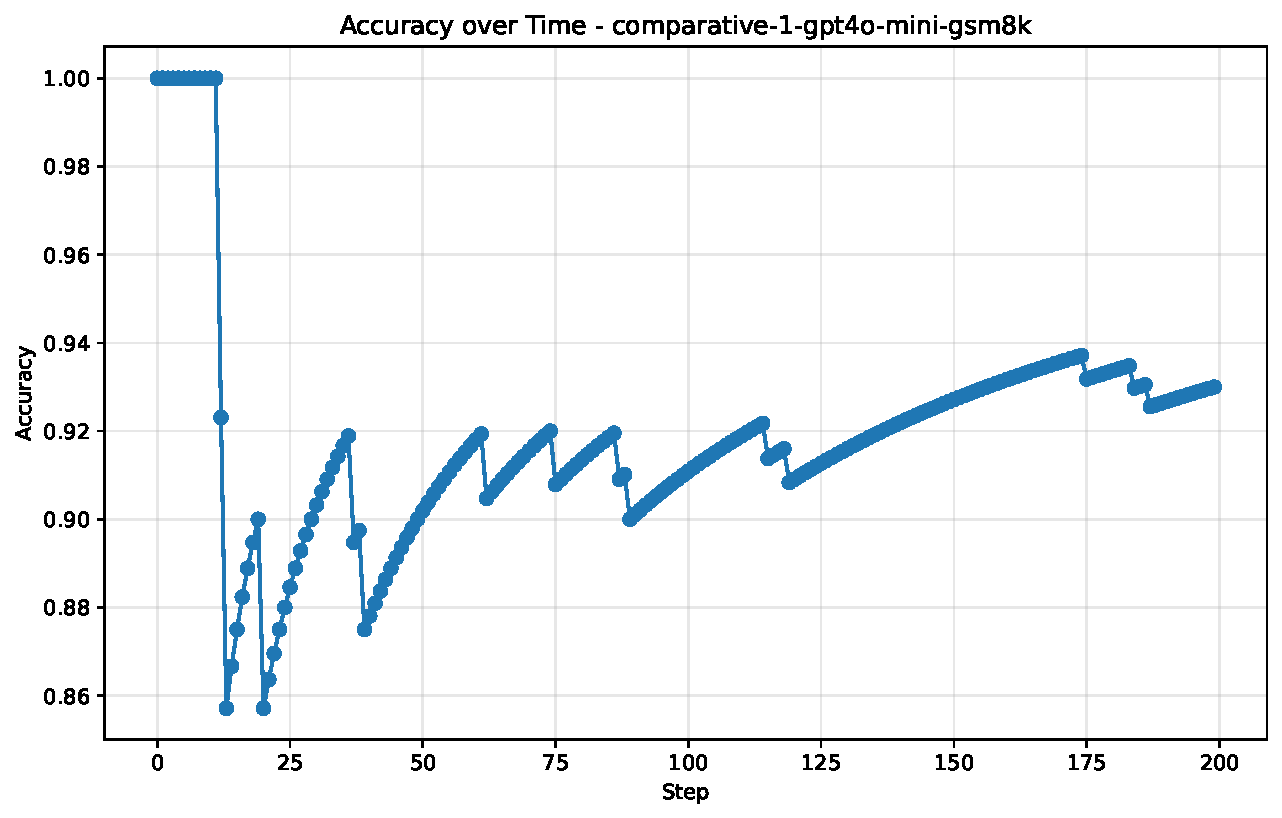
\includegraphics[width=0.7\linewidth]{images/comparative-1-gpt4o-mini-gsm8k_accuracy.pdf}
\caption{Accuracy over time for SC baseline on GSM8K ($N = 200$); higher values indicate better performance.}
\label{fig:gsm8k-sc-trace}
\end{figure}

\begin{figure}[H]
\centering
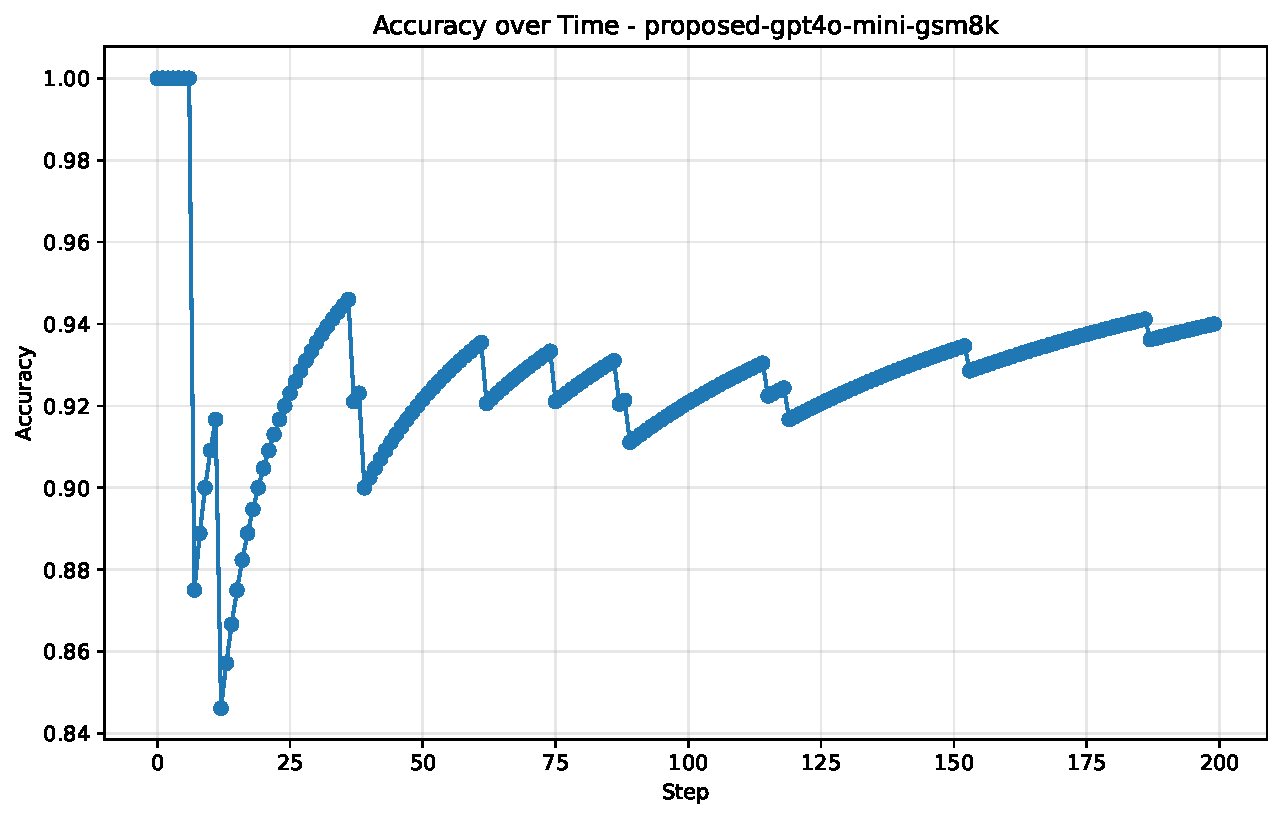
\includegraphics[width=0.7\linewidth]{images/proposed-gpt4o-mini-gsm8k_accuracy.pdf}
\caption{Accuracy over time for SFw-SC-CoT on GSM8K ($N = 200$); higher values indicate better performance.}
\label{fig:gsm8k-sfwsc-trace}
\end{figure}

\begin{figure}[H]
\centering
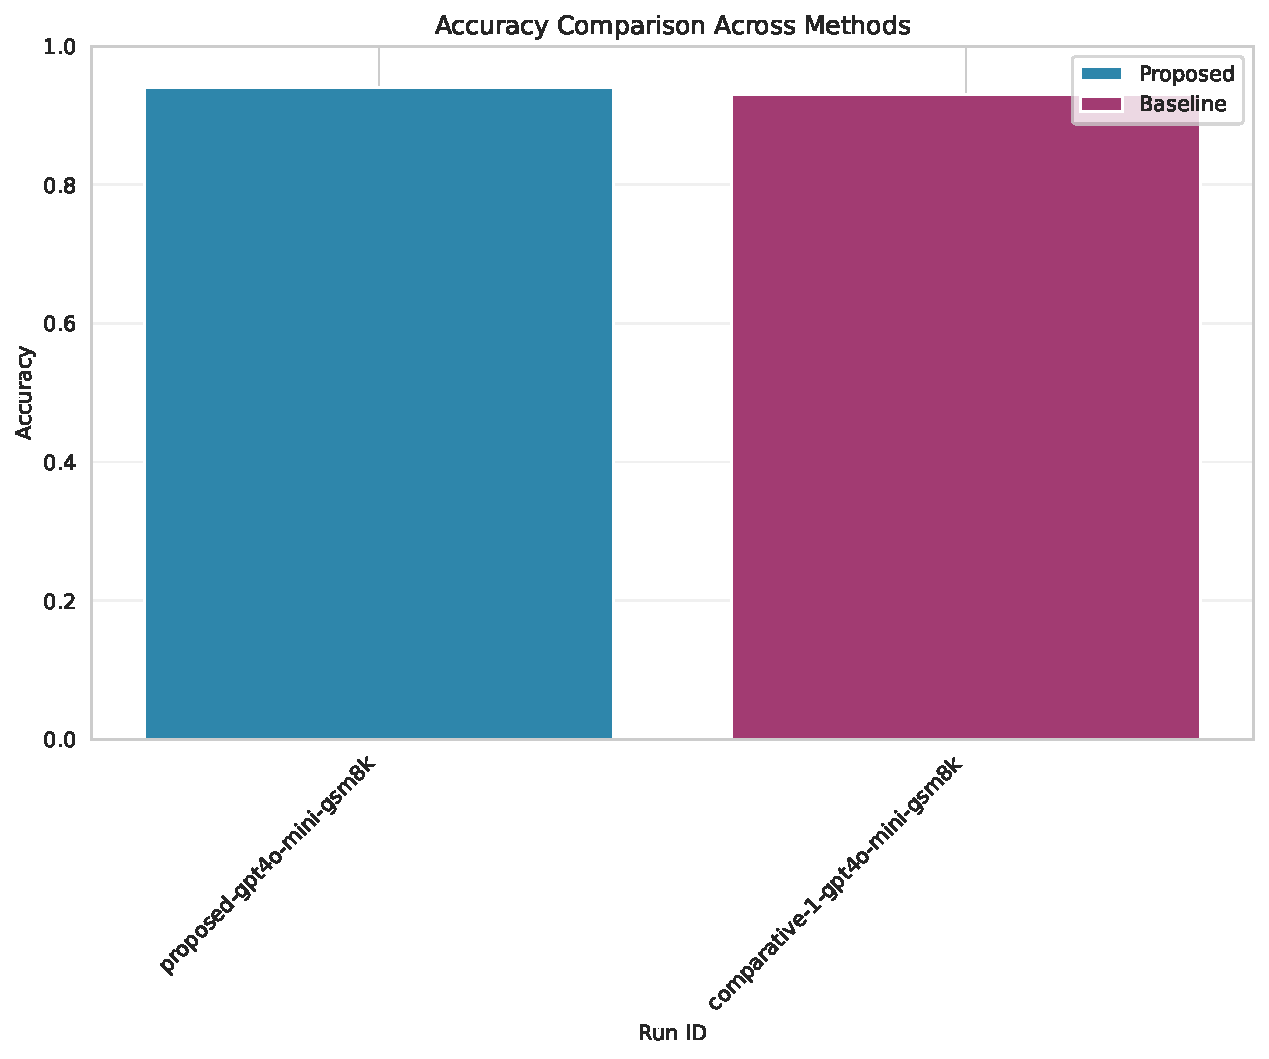
\includegraphics[width=0.7\linewidth]{images/comparison_accuracy.pdf}
\caption{Final accuracy comparison across methods on GSM8K ($N = 200$); higher values indicate better performance.}
\label{fig:gsm8k-accuracy-bar}
\end{figure}

\begin{figure}[H]
\centering
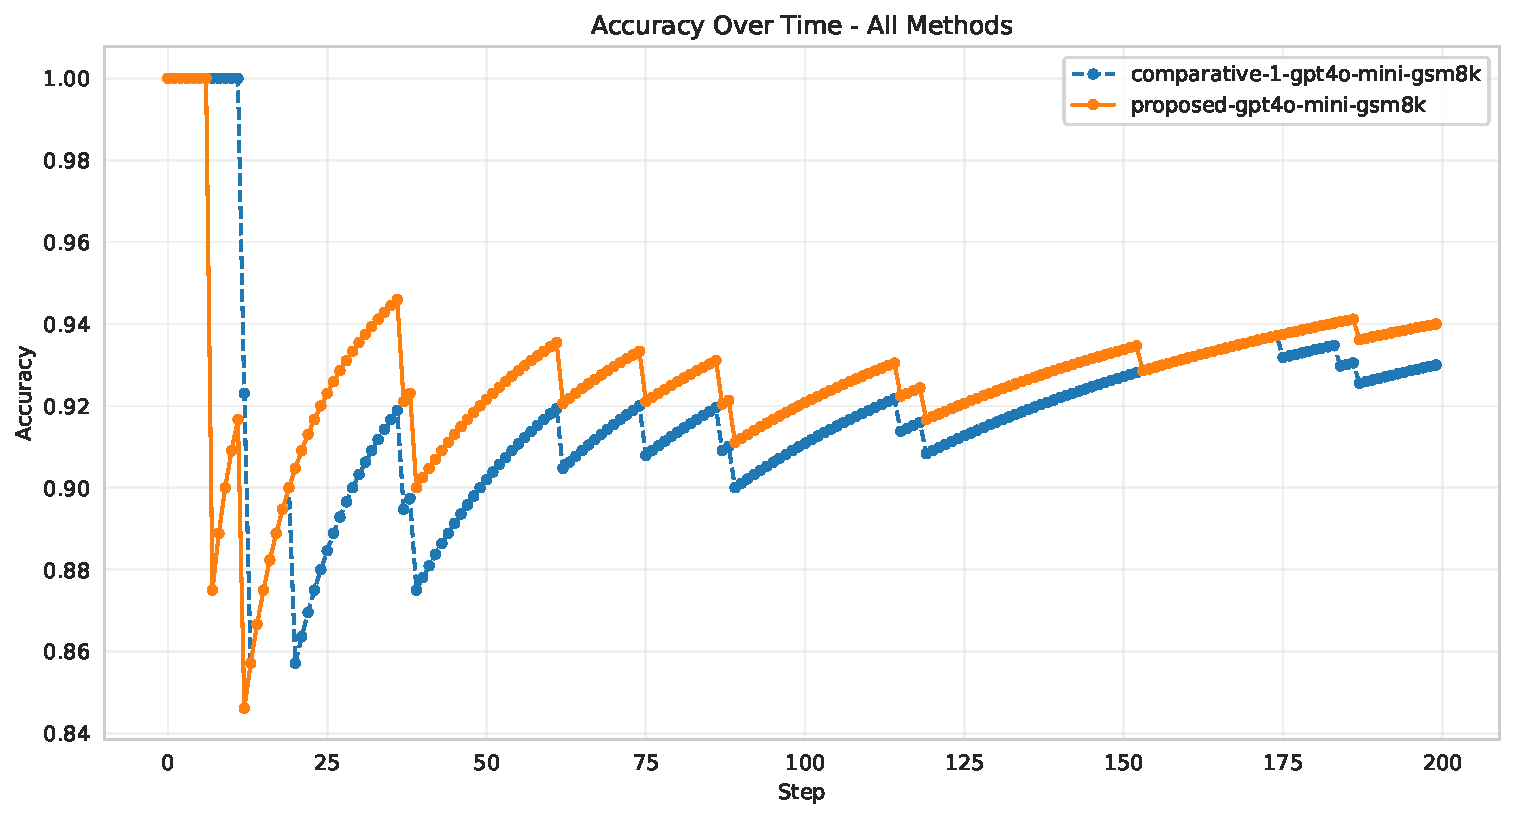
\includegraphics[width=0.7\linewidth]{images/comparison_accuracy_over_time.pdf}
\caption{Accuracy over time overlay for SC vs SFw-SC-CoT on GSM8K ($N = 200$); higher values indicate better performance.}
\label{fig:gsm8k-accuracy-overlay}
\end{figure}

The final accuracies visualized in Figure~\ref{fig:gsm8k-accuracy-bar} match the WandB summaries ($0.93$ for SC and $0.94$ for SFw-SC-CoT). The per-run traces (Figure~\ref{fig:gsm8k-sc-trace} and Figure~\ref{fig:gsm8k-sfwsc-trace}) and overlay plot (Figure~\ref{fig:gsm8k-accuracy-overlay}) report accuracy as examples are processed.

\subsection{Limitations evidenced by the results}
The experiments validate that SFw-SC-CoT can improve accuracy over SC in this specific setting, but they do not yet validate the proposed compute-efficiency motivation. The observed runtime increase, together with missing logs for $U$ and token usage, means we cannot demonstrate a budget-aware tradeoff empirically. Additionally, because verifier outputs (confidence and checks passed) are not logged, we cannot directly evaluate whether falsification signals are well calibrated or whether they discriminate correct versus incorrect answer hypotheses in the intended way.

%%%%%%%%%%%%%%%%%%%%%%%%%%%%%%%%%%%%%%%%%%
\section{Discussion}



%%%%%%%%%%%%%%%%%%%%%%%%%%%%%%%%%%%%%%%%%%
\section{Conclusions}

This paper examined a brittleness of standard self-consistency for chain-of-thought reasoning: majority voting treats sampled chains as exchangeable and uses answer frequency as a proxy for correctness, which can fail when samples share systematic misconceptions. To address this, we proposed Selective Falsification-Weighted Self-Consistency (SFw-SC-CoT), a prompt-only and inference-only method that clusters sampled chains by extracted final answer and verifies each unique answer hypothesis using a falsification-style checklist consisting of estimation, alternative recomputation, and constraint checking. The verifier produces a continuous confidence score and a discrete checks-passed signal, and these are combined with down-weighted frequency in a multiplicative scoring rule.

On GSM8K test problems ($N = 200$) using gpt-4o-mini with $K = 8$ sampled chains, SFw-SC-CoT improved accuracy from $0.93$ ($186/200$) to $0.94$ ($188/200$). This is a modest but positive directional improvement consistent with the idea that structured falsification can help resolve cases where frequency alone is misleading.

The current evaluation also highlights clear next steps. The logs do not report hypothesis counts, verifier-call counts, or token usage, and the observed runtime increase indicates that engineering and measurement are needed to substantiate the intended budget-aware benefits. Future work should expand the evaluation across datasets and sampling budgets and instrument the pipeline to quantify accuracy as a function of explicit compute cost, while retaining the prompt-only nature of the approach.

%%%%%%%%%%%%%%%%%%%%%%%%%%%%%%%%%%%%%%%%%%
\vspace{6pt}

%%%%%%%%%%%%%%%%%%%%%%%%%%%%%%%%%%%%%%%%%%
\authorcontributions{For research articles with several authors, a short paragraph specifying their individual contributions must be provided. The following statements should be used ``Conceptualization, X.X. and Y.Y.; methodology, X.X.; software, X.X.; validation, X.X., Y.Y. and Z.Z.; formal analysis, X.X.; investigation, X.X.; resources, X.X.; data curation, X.X.; writing---original draft preparation, X.X.; writing---review and editing, X.X.; visualization, X.X.; supervision, X.X.; project administration, X.X.; funding acquisition, Y.Y. All authors have read and agreed to the published version of the manuscript.'', please turn to the  \href{http://img.mdpi.org/data/contributor-role-instruction.pdf}{CRediT taxonomy} for the term explanation. Authorship must be limited to those who have contributed substantially to the work~reported.}

\funding{This research received no external funding.}

\dataavailability{All resources used in this study are openly available at }

\acknowledgments{In this study, we automatically carried out a series of research processes—from hypothesis formulation to paper writing—using generative AI.}

\conflictsofinterest{The authors declare no conflicts of interest.}

%%%%%%%%%%%%%%%%%%%%%%%%%%%%%%%%%%%%%%%%%%
%\isPreprints{}{% This command is only used for ``preprints''.
\begin{adjustwidth}{-\extralength}{0cm}
%} % If the paper is ``preprints'', please uncomment this parenthesis.
%\printendnotes[custom] % Un-comment to print a list of endnotes

\bibliographystyle{plainnat}
\bibliography{references}

\PublishersNote{}
%\isPreprints{}{% This command is only used for ``preprints''.
\end{adjustwidth}
%} % If the paper is ``preprints'', please uncomment this parenthesis.
\end{document}
